\chapter{Implementation}
\label{ch:implementation}

\section{Technology Stack}

\begin{table}[H]
\centering
\caption{FairLint-DL technology stack.}
\label{tab:techstack}
\begin{tabular}{@{}lll@{}}
\toprule
\textbf{Component} & \textbf{Technology} & \textbf{Purpose} \\
\midrule
DNN Framework & PyTorch 2.0+ & Model training, gradient computation \\
Backend Server & FastAPI + Uvicorn & REST API, async request handling \\
Extension Frontend & TypeScript & VS Code extension, WebView dashboard \\
Data Visualization & Plotly.js (CDN) & Interactive charts in WebView \\
Data Processing & Pandas, Scikit-learn & CSV loading, encoding, scaling \\
Explainability & SHAP, LIME & Feature attribution \\
\bottomrule
\end{tabular}
\end{table}

\section{DNN Model Architecture}

The \texttt{FairnessDetectorDNN} class implements a configurable feedforward neural network:

\begin{lstlisting}[language=Python, caption={DNN architecture definition (simplified).}]
class FairnessDetectorDNN(nn.Module):
    def __init__(self, input_dim, hidden_layers=[64,32,16,8,4],
                 num_classes=2, dropout=0.2):
        super().__init__()
        layers = []
        prev_dim = input_dim
        for h in hidden_layers:
            layers.extend([
                nn.Linear(prev_dim, h),
                nn.BatchNorm1d(h),
                nn.ReLU(),
                nn.Dropout(dropout)
            ])
            prev_dim = h
        layers.append(nn.Linear(prev_dim, num_classes))
        self.network = nn.Sequential(*layers)
\end{lstlisting}

For the Adult Census dataset with 14 features, the model contains 3,998 trainable parameters across layers $\langle 64, 32, 16, 8, 4, 2 \rangle$.

\section{Model Caching System}

To avoid redundant retraining, FairLint-DL implements a deterministic SHA-256 caching system. The cache key is computed from six parameters: the SHA-256 hash of the CSV file contents (not the file path), the label column name, the sorted set of sensitive features, hidden layer sizes, number of epochs, and batch size. Any change to these parameters invalidates the cache. Stored artifacts include model weights (\texttt{model.pt}), preprocessor state (\texttt{preprocessor.pkl}), train/validation/test data splits (\texttt{data\_tensors.pt}), and human-readable metadata (\texttt{metadata.json}).

\section{Data Preprocessing}

The \texttt{data\_loader.py} module handles CSV loading with automatic type detection: categorical features are ordinally encoded, continuous features are standardized via \texttt{StandardScaler} (zero mean, unit variance), and the dataset is split into training (70\%), validation (10\%), and test (20\%) partitions. Protected attributes are auto-detected via regex pattern matching against common sensitive feature names (age, gender, sex, race, ethnicity, religion, disability, national origin, marital status).

\section{VS Code Extension Integration}

The extension is activated on Python files or workspaces containing CSV files. Users trigger analysis via the context menu (right-click on a \texttt{.csv} file). The extension presents QuickPick dialogs for selecting the label column, protected attributes, and model architecture. Configurable settings are exposed through VS Code's settings API, including training epochs (default: 30), batch size (default: 32), hidden layer configuration, QID threshold (default: 0.1 bits), maximum analysis samples (default: 500), server port, and visualization theme.

\begin{figure}[H]
    \centering
    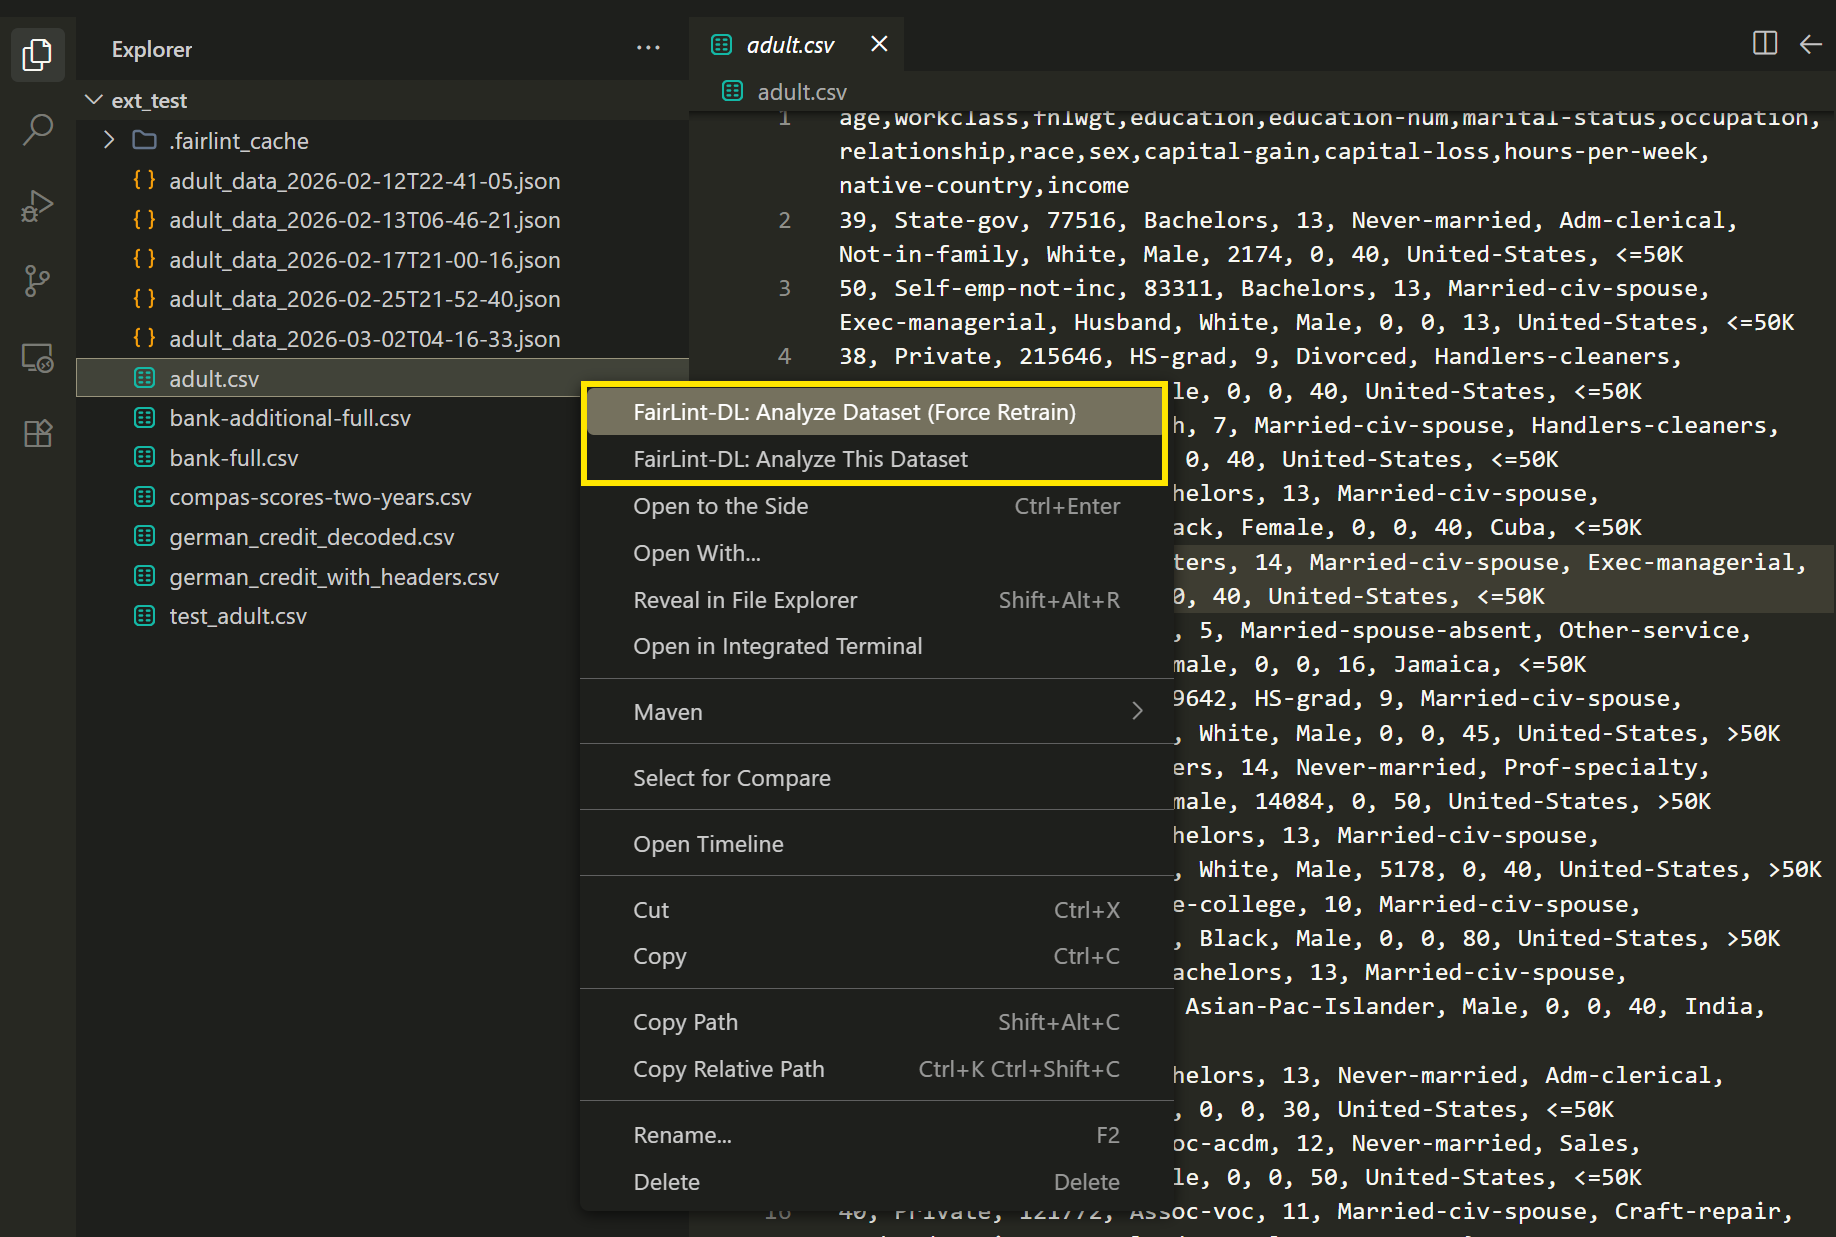
\includegraphics[width=0.95\textwidth]{images/context-menu-vscode.png}
    \caption{FairLint-DL context menu integration in VS Code.}
    \label{fig:vscode_menu}
\end{figure}
